% !TEX spellcheck = en_US
%=================================================================================
\chapter{Controller tuning}

In this chapter first calculated the steady-state value to initialize the simulation. After that, the focus to DEL calculation and parameter optimization, minimum pitch angle and the minimum pitch angle optimization for control region 1.5.


%=================================================================================
\section{Steady States (Soni)} \label{steady states}
% !TEX spellcheck = en_US

The steady states are influenced by the design of the controller and turbine in the simulation. These states are useful for initializing the simulation, as they provide essential information for analyzing the turbine's power behavior and the controller settings. Additionally, these steady states play a crucial role in the overall wind turbine design and can be utilized to initialize further simulations.
\\[16pt]


\section{DEL calculations and Parameter Optimization (Felix)} \label{DLC 1.2 tuning}
% !TEX spellcheck = en_US
% Parameter Optimization
%=================================================================================
To optimize the controller and its parameters such as $k$ in Control-Region 2, $k_p$ for the pitch control in Control-Region 3, $\Delta P$ in Control-Region 2.5 and $\theta_k$ in Control-Region 3, a Brute-force optimization pattern has been followed.

The used method runs the DLC 1.2 for the selected control parameter for a specified range of the control value. Used wind disturbance is created beforehand with the use of \textbf{TurbSim} and the GenerateTurbSimWindFields.m file from the SummerGames. The input parameter to \textbf{TurbSim} that has been changed are the turbulence class is set to \textit{B} and the grid values to math the dimensions of the Shakti WT. The wind time series are created in a range of $[4:2:24]\frac{m}{s}$ with $6$ different Seeds per wind speed. The length of the series are $T = \SI{600}{s}$. In the DLC calculation the simulation is done $6$ times per wind speed for all diferent seeds and also for all $12$ wind speeds to ensure a simulation Time per wind speed of $T_{\text{Simulation}} = \SI{3600}{s}$. With this setup the Overspeed, Life time weighted Damage Equivalent Loads (DEL) and the Anual Energy Production (AEP) is computed. The used Weibull parameter for the lifetime weighting are $C = \frac{2}{\sqrt{\pi}}\cdot7.5$, this corresponds to the wind class \MakeUppercase{\romannumeral 3} \cite{IEC61400-1} and a $k = 2$. Equation \ref{eq:Weibull} shows how the Weibull distribution is computed in this case.
\begin{equation}
	f(V_{\text{ref}}) = \frac{k}{C}\left(\frac{V_{\text{ref}}}{C}\right)^{k-1} \exp\left(-\left(\frac{V_{\text{ref}}}{C}\right)^k\right)
	\label{eq:Weibull}
\end{equation}
The weighting function is derived to \ref{eq:Weighting}
\begin{equation}
	w(V_{\text{ref}}) = \frac{f(V_{\text{ref}})}{\sum f(V_{\text{ref}})}
	\label{eq:Weighting}
\end{equation}
The AEP is calculated as \ref{eq:AEP}
\begin{equation}
	AEP = \sum \left(\bar{P}_{\text{el}}w(V_{\text{ref}})\right)\cdot \SI{8760}{h}
	\label{eq:AEP}
\end{equation}
The DEL calculation is using the parameters of the Woehler-Exponent as $m = 4$ hence this is the typical value for steel a reference number of $N_{\text{ref}} = \frac{2\cdot10^6}{20\cdot8760}$ as a value for 20 years for 1 hour simulations.
The DEL is calculated per $V_{\text{ref}}$ with the use of the rainflow count as $\text{DEL}(V_{\text{ref}})$ and the life time weighted DEL is than calculated in \ref{eq:LTW-DEL}.
\begin{equation}
	\text{DEL}_{\text{LTW}} = \left(w(V_{\text{ref}})\text{DEL}(V_{\text{ref}})^m\right)^{\frac{1}{m}} 
	\label{eq:LTW-DEL}
\end{equation}
The parameters $\Delta P$ in Control-Region 2.5 and  $k$ in Control-Region 2 are optimized first hence they are not depending on another control parameter. Figure \ref{fig:DeltaP} shows one example of how the optimization results are displayed. The chosen control parameter is $\Delta P = \SI{4.9}{MW}$ hence the AEP is higher than for $\Delta P = \SI{4.9}{MW}$ without a change in the life time weighted DEL.
\begin{figure}[tbh]
	\centering	
	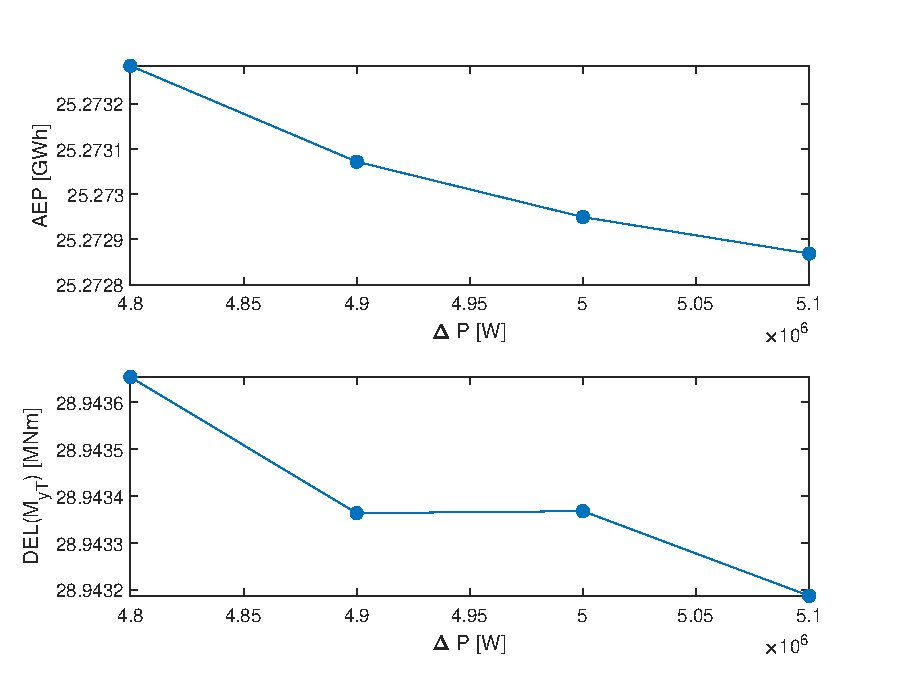
\includegraphics[width=12cm]{Figures/DeltaPopt.eps}
	\caption{Brute-Force optimization of $\Delta P$}
	\label{fig:DeltaP}
\end{figure}

\section{Minimum Pitch Angle Optimization (Julius)} \label{minimum pitch angle static}
% !TEX spellcheck = en_US
% Theta min static calculations
The optimization of the minimum pitch angle is a simple adjustment which leads to a small increase in the AEP. 
The optimization was done with a brute force approach and the steady states calculations (Section \ref{steady states}). 
In control region 2 the WT should work at optimum $Cp$ and $\lambda$. 
The use of minimum pitch angle can lead to an more efficient state of the turbine at the start of region 2 and therefor increase the AEP. 
For different pitch angles the steady states where calculated. 
As optimum, min. pitch angle the angle which leads to the highest $Cp$ was chosen. 
As a result the min. pitch angle of \SI{0.5}{\degree} was determined and is shown in figure \ref{fig:theta min general}. 
During the calculation the pitch angle was optimized in a range of \SI{0}{\degree} to \SI{5}{\degree} with a step size of \SI{0.1}{\degree}.

The determined min. pitch angle leads to an increase in AEP of \SI{0.29}{\%}. 
(Calculated with Weibull parameters of TC III and $k=2$.)

\begin{figure}[h]
	\centering	
	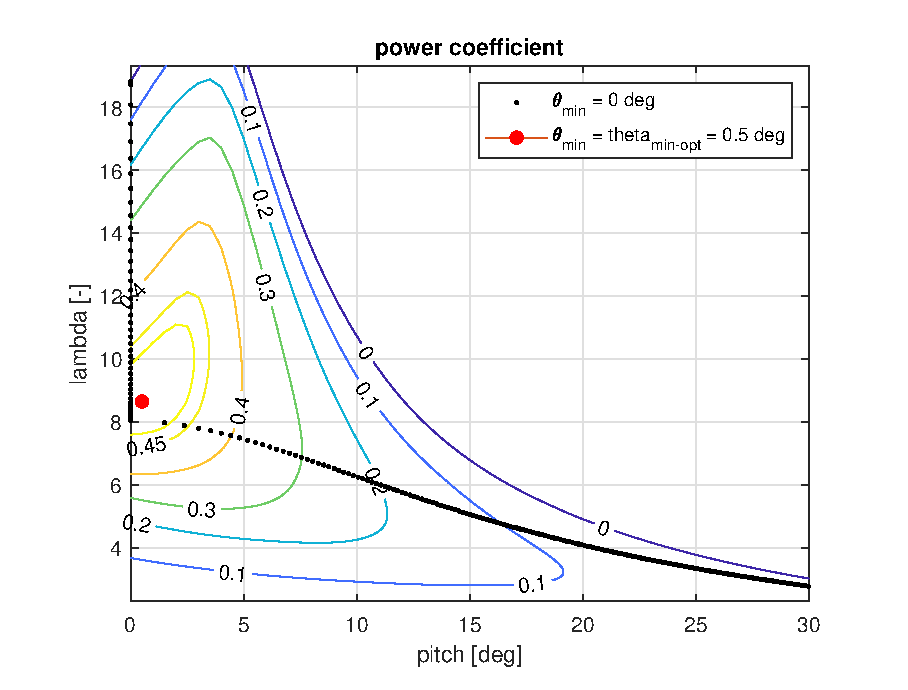
\includegraphics[width=12cm]{Figures/ThetaMinOpt.eps}
	\caption{brute force optimization for minimum pitch angle $\theta$}
	\label{fig:theta min general}
\end{figure}

\section{Minimum Pitch Angle Optimization for Control Region 1.5 (Julius)} 
% !TEX spellcheck = en_US
% Theta min dynamic calculations
%=================================================================================
Since the control region 1.5 has a large wind speed range of \SI{3.36}{m/s} the optimization of the pitch angle could lead to an increase in AEP.
As optimization process a brute force approach was used in order to find the optimum pitch angle for every operating wind speed in region 1.5. 
During the calculation the pitch angle was optimized in a range of \SI{0}{\degree} to \SI{5}{\degree} with a step size of \SI{0.1}{\degree}. 
The results of the optimization can be seen in Figure \ref{fig:theta min dynamic}. 
The result shows, that keeping a static pitch angle through region 1.5 is not leading to the optimal power production. 
A calculation of the AEP with a dynamic pitch adjustment for region 1.5 leads to an increase of \SI{0.19}{\%} compared to a static minimum pitch angle of \SI{0.5}{\degree} as shown in section \ref{minimum pitch angle static}.
(Calculated with Weibull parameters of TC III and $k=2$.)
Since the calculation is done without transition regions for the adjustment of the pitch the increase in AEP after implementation of the control behavior is to be expected less than the named \SI{0.19}{\%}.
The approach of changing the pitch angle dynamically in region 1.5 was not implemented in the \gls{shakti} project but could be interesting for further optimization of the developed WT.  

\begin{figure}[h]
	\centering	
	\includegraphics[width=12cm]{Figures/ThetaMinOptDynamic}
	\caption{Brute force optimization for minimum pitch angle $\theta$ in region 1.5}
	\label{fig:theta min dynamic}
\end{figure}
